\documentclass[11pt,reqno]{article}
\usepackage{amsmath,amssymb,mathrsfs,amsthm}
\usepackage[UTF8]{ctex}
%\usepackage{xeCJK}
%\setCJKmainfont{SimSum}

\usepackage{graphicx,cite,cases}
%\usepackage[pagewise]{lineno}\linenumbers
%\usepackage{refcheck}
\usepackage{xcolor}
\usepackage{bm}			% 公式加粗
\usepackage{tabularx}   % 绘制定宽表格
\usepackage{dcolumn}	% 表格横向合并
\usepackage{multirow}	% 表格纵向合并
\usepackage{booktabs}	% 三线表
\usepackage{authblk}	% 添加更多作者信息
\usepackage{appendix} 	% 生成附录
\usepackage{listings}   % 附录里的代码, 支持语言高亮
\usepackage{hyperref}   % 超链接, 自动跳转
\usepackage{subfigure}  % 插入多张图片
\usepackage{tikz}		% 代码作图


\setlength{\topmargin}{-1.5cm}
\setlength{\oddsidemargin}{0.0cm}
\setlength{\evensidemargin}{0.0cm}
\setlength{\textwidth}{16.7cm}
\setlength{\textheight}{23cm}
\headheight 20pt
\headsep    26pt
\footskip 0.4in

%%%%% 关于公式编号问题 %%%%%
%统一用equation环境
%如果需要加括号用\begin{cases}
%如果公式过长需要分行用\begin{split}
%如果一个equation里面需要多个公式, emmm没研究过

\newtheorem{theorem}{Theorem}[section]
\newtheorem{corollary}[theorem]{Corollary}
\newtheorem{lemma}[theorem]{Lemma}
\newtheorem{proposition}[theorem]{Proposition}
\newtheorem{remark}[theorem]{Remark}
\newtheorem{definition}[theorem]{Definition}
\numberwithin{equation}{section}


\renewcommand{\d}{\,\mathrm d}
\usepackage{algorithm,algorithmicx}  %写伪代码
\usepackage{algpseudocode}			% 写伪代码
%%%%%% 算法部分改为中文显示 %%%%%%%%%
%%\floatname{algorithm}{算法}
\renewcommand{\algorithmicrequire}{\textbf{Input:}}
\renewcommand{\algorithmicensure}{\textbf{Output:}}

%% Ctrl+Alt+R 编译
%% Ctrl+Alt+V 打开文档

\begin{document}

\title{微分方程数值解计算实习Lecture 8}

\author{朱荃凡}
\affil{(吉林大学数学系计算唐班)}
\date{\today}

\maketitle

\vspace{50pt}

如图所示,\ $\Omega$表示$[0,1]^2$的区域,\ $\Gamma_1,\Gamma_2,\Gamma_3,\Gamma_4$
是它的四条边:
\begin{center}
	\begin{tikzpicture}[scale=2.5]
		% 绘制坐标轴
		\draw[->] (-0.2,0) -- (1.3,0) node[below] {$x$};
		\draw[->] (0,-0.2) -- (0,1.3) node[left] {$y$};
		% 绘制坐标轴标签
		\foreach \x in {}
			\draw (\x,0.05) -- (\x,-0.05) node[below] {$\x$};
		\foreach \y in {}
			\draw (0.05,\y) -- (-0.05,\y) node[left] {$\y$};
		% 绘制矩形
		\draw[fill=gray!20] (0,0) rectangle (1,1);
		\node[below left] at (0,0){$O$};
		\node[below] at (1,0){$(1,0)$};
		\node[left] at (0,1){$(0,1)$};
		\node[right] at (1,1){$(1,1)$};
		\node[above right] at (0.4,0.4){$\Omega$};
		\node[left] at (0,0.5){$\Gamma_1$};
		\node[right] at (1,0.5){$\Gamma_2$};
		\node[below] at (0.5,0){$\Gamma_3$};
		\node[above] at (0.5,1){$\Gamma_4$};
	\end{tikzpicture}
\end{center}
利用三角剖分线性元元求解区域$\Omega$区域上的偏微分问题:
\begin{equation}\label{Eqn1}
	\left\{\begin{matrix}
		-\Delta u-2\pi^2u=-2\pi^2xy,&\mathrm{in}\ \Omega,\\
		u(x,y)=0,&\mathrm{in}\ \Gamma_1,\Gamma_3,\\
	   \partial_x u(x,y)=y-\pi\sin(\pi y),&\mathrm{in}\ \Gamma_2,\\
	   \partial_y u(x,y)=x-\pi\sin(\pi x),&\mathrm{in}\ \Gamma_4.
	   \end{matrix}\right.
\end{equation}
其相应的的真解为
\begin{equation}
	u^*=xy+\sin(\pi x)\sin(\pi y).
\end{equation}
求数值解的网点$C-$范数和$0-$范数误差并画出误差图.

\newpage

\section{算法设计}

在课件中给出了边值条件的两种的处理方式——数值微商法和有限体积法.使用同样的方式,可以得到
右上顶角处的方程.

数值微商法:
\begin{equation}
	\begin{split}
	\left[\frac{u(x_{N-1},y_N)-u(x_N,y_N)}{h^2}\right]+
	\left[\frac{u(x_N,y_{N-1})-u(x_N,y_N)}{h^2}\right]
	+q(x_N,y_N)u(x_N,y_N)\\
	=f(x_N,y_N)-\frac{1}{h}\left(u_x(x_N,y_N)+u_y(x_N,y_N)\right).
	\end{split}
\end{equation}

有限体积法:
\begin{equation}
	\begin{split}
	\left[\frac{u(x_{N-1},y_N)-u(x_N,y_N)}{2h^2}\right]+
	\left[\frac{u(x_N,y_{N-1})-u(x_N,y_N)}{2h^2}\right]
	+\frac{1}{4}q(x_N,y_N)u(x_N,y_N)\\
	=\frac{1}{4}f(x_N,y_N)-\frac{1}{2h}\left(u_x(x_N,y_N)+u_y(x_N,y_N)\right).
	\end{split}
\end{equation}
\vspace{50pt}

\section{程序结果}

\subsection{不同边值方法下的误差}

建于数值解和真解的图像我们已经在往期报告中看过许多次了,这回换一种表现方式.

在此问题中,我们使用均匀剖分.设剖分数为$N$,此时x轴和y轴均被$N$等分,\ 区域$\Omega$
上有$N^2$个小正方形单元和$(N+1)^2$个剖分节点,也就是自由度. 当$N=4$时,剖分如下所示
\begin{center}
	\begin{tikzpicture}[scale=4]
		% 绘制坐标轴
		\draw[->] (-0.1,0) -- (1.2,0) node[below] {$x$};
		\draw[->] (0,-0.1) -- (0,1.2) node[left] {$y$};
		% 绘制坐标轴标签
		\foreach \x in {}
			\draw (\x,0.05) -- (\x,-0.05) node[below] {$\x$};
		\foreach \y in {}
			\draw (0.05,\y) -- (-0.05,\y) node[left] {$\y$};
		% 绘制矩形
		\draw[fill=gray!20] (0,0) rectangle (1,1);
		% 绘制剖分
		\draw (0.25,0) -- (0.25,1);
		\draw (0.5,0) -- (0.5,1);
		\draw (0.75,0) -- (0.75,1);
		\draw(0,0.25) -- (1,0.25);
		\draw(0,0.5) -- (1,0.5);
		\draw(0,0.75) -- (1,0.75);
		% 节点编号
		\foreach \x in {0,1,2,3,4} {
    	\foreach \y in {0,1,2,3,4} {
		\pgfmathtruncatemacro{\z}{(\x)*5+\y+1} % 计算节点序号
		\pgfmathsetmacro{\xx}{\x*0.25} % 计算节点序号
		\pgfmathsetmacro{\yy}{\y*0.25} % 计算节点序号
      	\filldraw (\xx,\yy) circle (0.5pt) node[left] 
		{\footnotesize{\textit{\z}}};}}
		% 区间编号
		\foreach \x in {1,2,3,4} {
    	\foreach \y in {1,2,3,4} {
		\pgfmathtruncatemacro{\z}{\x*4-4+\y} % 计算节点序号
		\pgfmathsetmacro{\xx}{\x*0.25-0.19} % 计算节点序号
		\pgfmathsetmacro{\yy}{\y*0.25-0.175} % 计算节点序号
      	% 标记节点
      	\node[above right] at (\xx,\yy){\small{\textbf{\z}}}; }}
	\end{tikzpicture}
\end{center}


取剖分数$N=10k(1\le k\le 10),$分别计算出两种边值条件处理方式下的数值解与真解的
$||\cdot||_C$误差和$||\cdot||_0$误差.得到如下表格.

比较奇怪的一点是数值微商法居然比有限体积法拥有更高的精度, 难道是我公式推导有问题?

\newpage

\begin{table}[h]\label{table1}
	\begin{center}
	\caption{\zihao{5}{数值解和真解的误差}}
	\begin{tabular}{c|c|c|c|c}
		\toprule
		\multirow{2}*{自由度} & \multicolumn{2}{c|}{数值微商法} 
						    &  \multicolumn{2}{c}{有限体积法} \\ \cline{2-5}
		& $\ ||\cdot||_C$误差\ & $\ ||\cdot||_0$误差\ & $\ ||\cdot||_C$\ 误差 
		& $\ ||\cdot||_0$误差\ \\ \hline
		100	&	0.01875	&	0.02958	&	0.02688	&	0.04655	\\
		400	&	0.00643	&	0.01459	&	0.00737	&	0.01675	\\
		900	&	0.00304	&	0.00851	&	0.00345	&	0.00922	\\
		1600	&	0.00175	&	0.00570	&	0.00200	&	0.00603	\\
		2500	&	0.00114	&	0.00415	&	0.00130	&	0.00433	\\
		3600	&	0.00082	&	0.00319	&	0.00091	&	0.00331	\\
		4900	&	0.00061	&	0.00255	&	0.00068	&	0.00263	\\
		6400	&	0.00048	&	0.00210	&	0.00052	&	0.00216	\\
		8100	&	0.00038	&	0.00177	&	0.00041	&	0.00181	\\
		10000	&	0.00031	&	0.00152	&	0.00034	&	0.00155 \\
		\bottomrule
	\end{tabular}
	\end{center}
\end{table}

\subsection{收敛阶}

两种边值方法的收敛阶是一样的, 这边以有限体积法为例.可以看出$||\cdot||_C$误差的收敛速度
为二阶, $||\cdot||_0$误差的收敛速度为$1.5$阶,可见收敛速度和维度有关.
\begin{figure}[h]
	\centering
		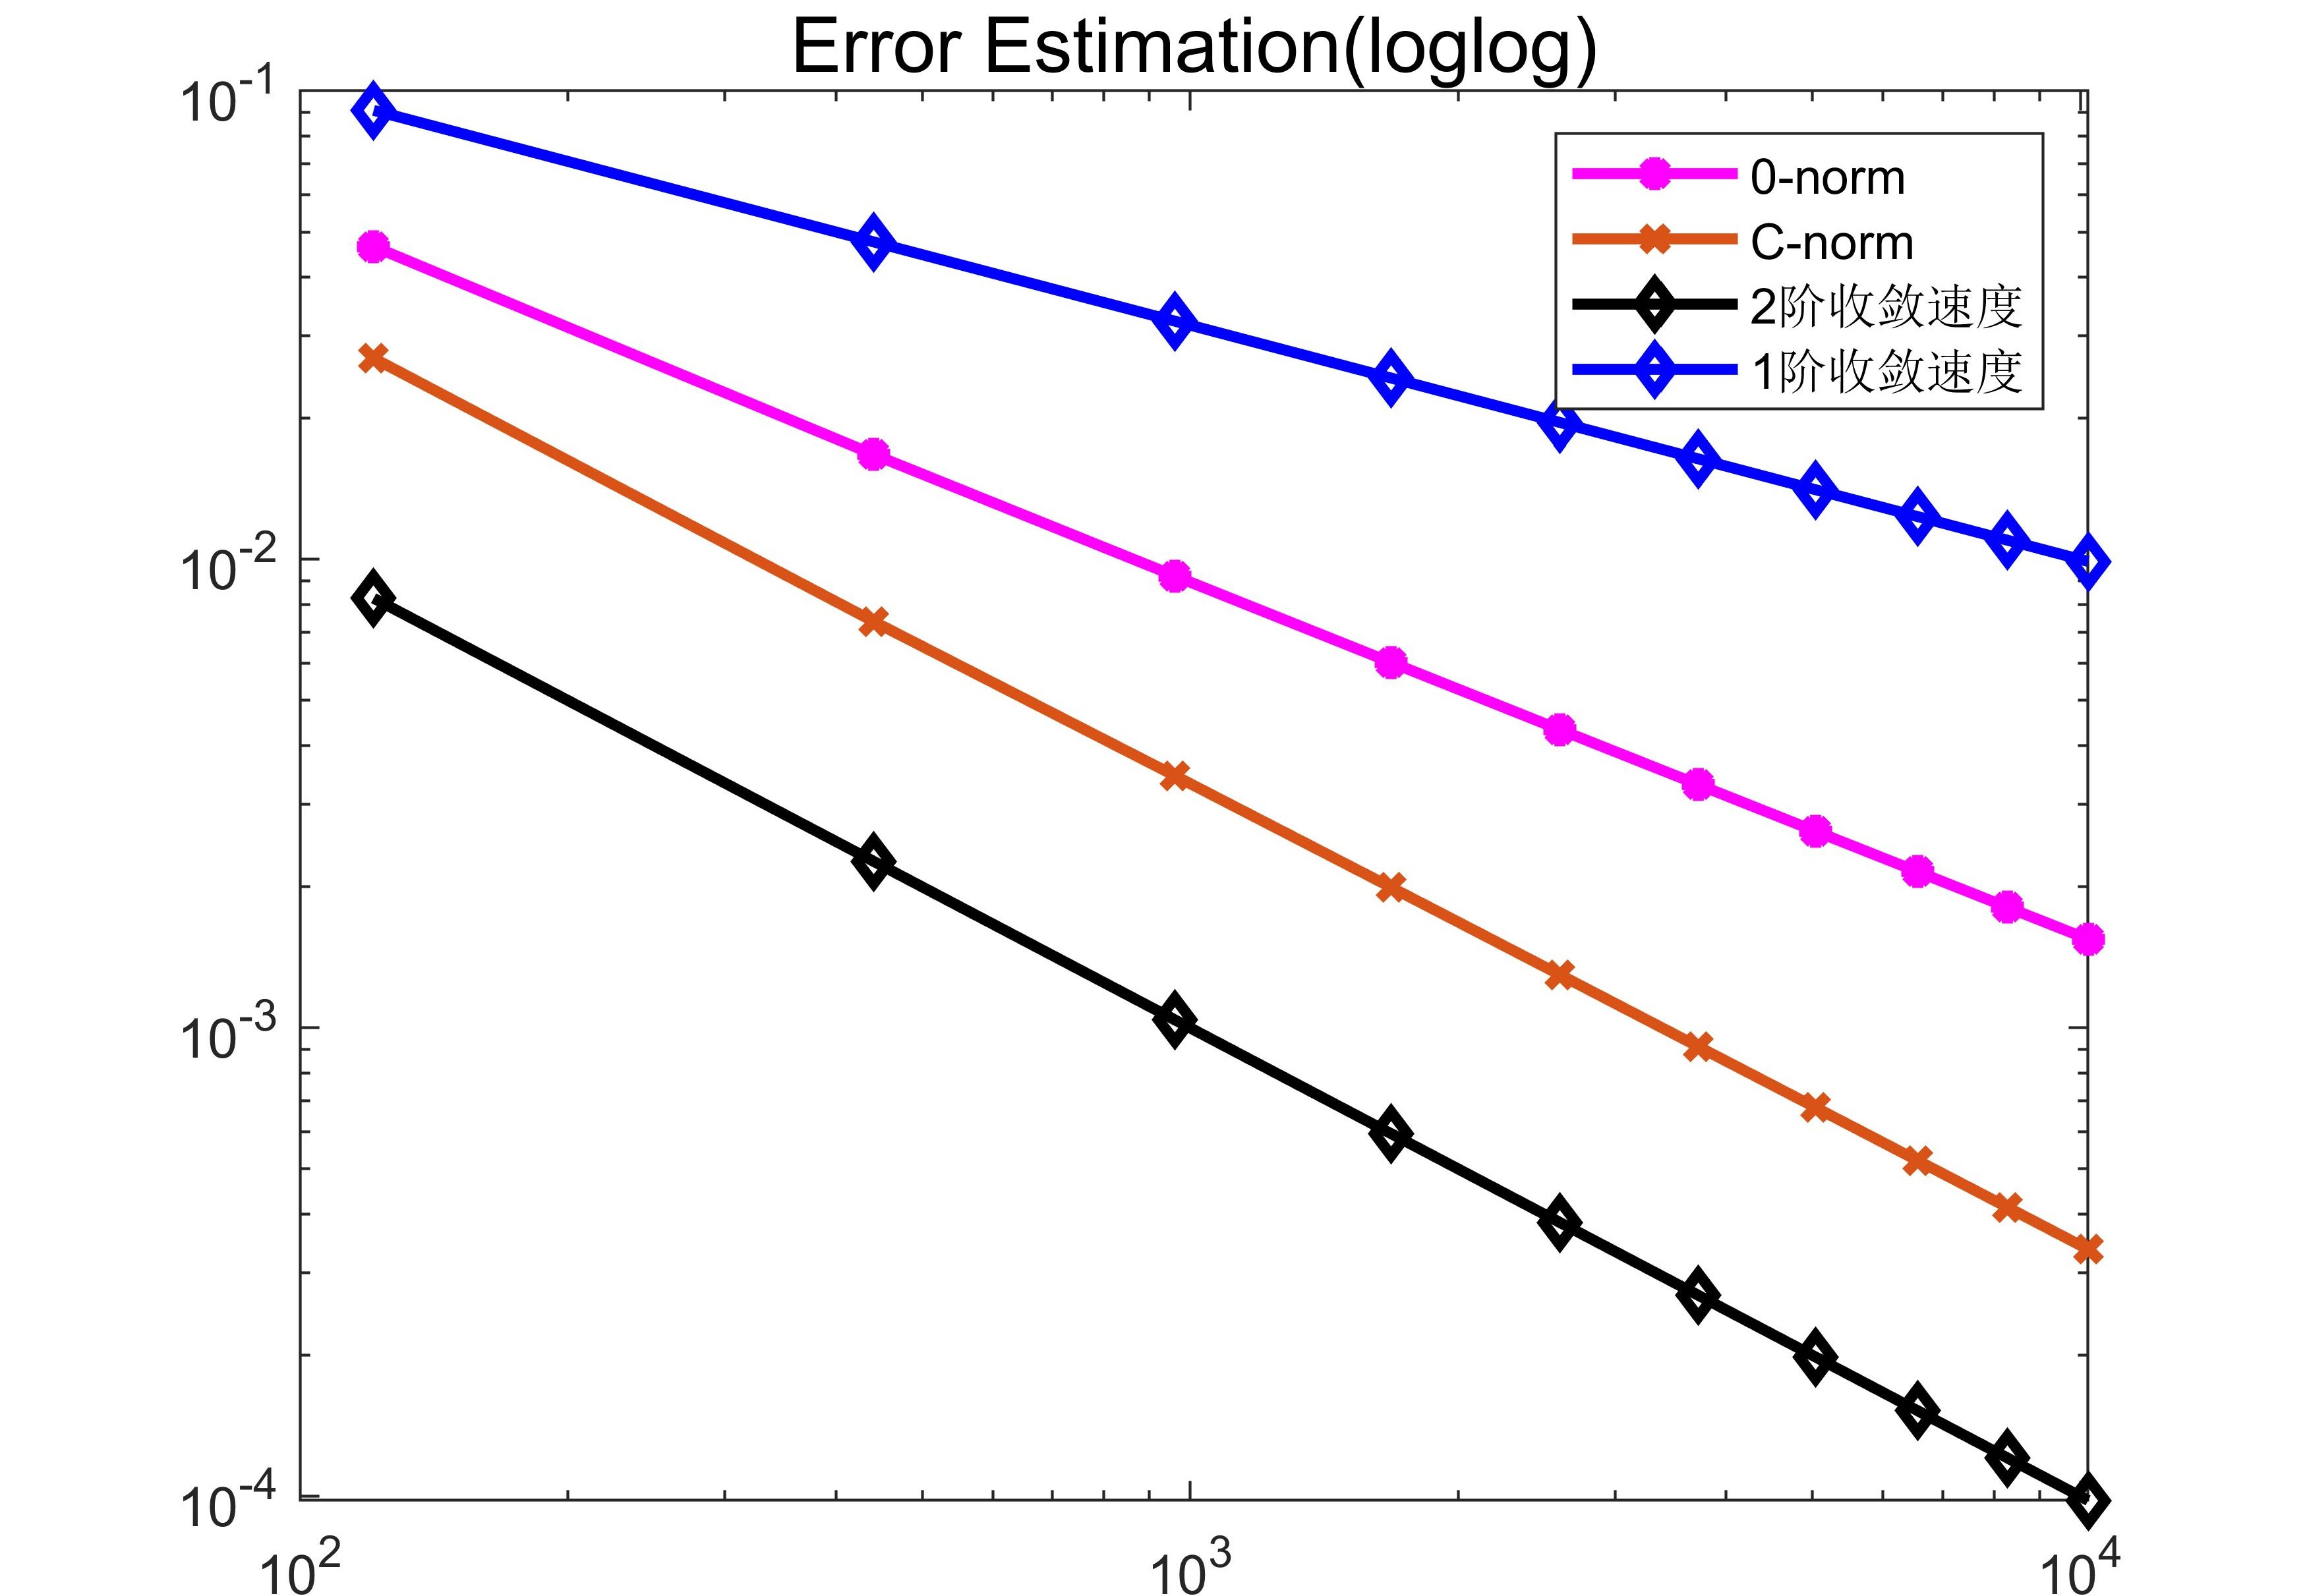
\includegraphics[width=0.7\textwidth]{Error.jpg}
\end{figure}


\end{document}
